\section{Experiments}

We evaluate \DynaSCSH across fixed-query synthetic configurations and a separate hybrid benchmark, targeting three questions: (Q1) What is the average-case speedup over static recomputation? (Q2) What happens when deletions force fallback-dominated behavior? (Q3) Does the framework scale to 100K-edge graph sizes?

\subsection{Experimental Setup}
\label{sec:setup}

\textbf{Evaluation settings.} We report two evidence-backed graph settings:
\begin{enumerate}
\item \textbf{Synthetic DBLP}: compact DBLP-like network with planted dense groups, used for all 22 fixed-query configurations.
\item \textbf{Hybrid} (26,850 nodes, 128,227 edges): 40 dense planted communities injected into the real 26K-node MAGNN DBLP graph~\cite{fu2020magnn}. This setting tests whether the \mtindex and repair machinery remain practical on a 100K-edge topology with guaranteed valid communities.
\end{enumerate}

\textbf{Update model.} The implementation maintains communities over the source-type graph induced by a symmetric meta-path, e.g., Author--Author projected edges under APA. This matches the edge set on which $(k,\mathcal{P})$-truss support is defined. Raw HIN relation updates such as Author--Paper insertions can change many projected source edges; supporting them incrementally requires a projection-refresh layer and is outside the per-source-edge complexity claim.

\textbf{Baselines and internal fairness.} We compare against \textbf{Static Recompute}: greedy heuristic community search from scratch after each update, equivalent to Zhang et al.'s polynomial-time baseline~\cite{zhang2025scsh}. Both the static baseline and \DynaSCSH's fallback path preserve the \emph{same original query node} throughout an update stream. This fixed-query condition is essential: using an endpoint of the latest update as the recomputation query can create artificial Jaccard divergence and invalid quality comparisons. Under the fixed-query design, the reported speedup measures the benefit of incremental maintenance against the exact algorithm the system itself would run if incrementality were disabled. Using exact B\&B as the baseline would compare a polynomial-time incremental method against an exponential-time oracle, mixing the effect of algorithmic choice with the effect of incrementality. As \DynaSCSH is the first dynamic approach for \emph{size-constrained} HIN communities, no existing dynamic baselines (e.g., CS-DAHIN~\cite{song2024tkde}) can enforce the exact cardinality constraint $|C|=s$; they produce communities of variable size, and post-hoc truncation violates the $(k,\mathcal{P})$-truss condition.

\textbf{Metrics.} (1) \textbf{Speedup}: ratio of static baseline latency to \DynaSCSH latency; (2) \textbf{\qratio}: $\text{score}_{\text{DynaSCSH}} / \text{score}_{\text{static}}$---measures relative community cohesiveness; (3) \textbf{Jaccard similarity}: structural overlap between maintained and recomputed communities.

\textbf{Environment.} Python 3.10, networkx 3.4.2, NumPy 2.2.6, single machine (Intel Core i7-13700, 32\,GB DDR5 RAM). All experiments are CPU-only. Each nonempty synthetic run uses 3 query nodes, 500--1,000 updates, and checkpoints every 10\% of the stream. The artifact includes the experiment runner and a post-fix invariant smoke script that checks fixed-query recomputation, \mtindex co-triangle updates, and community validation.

\textbf{Fast-path interpretation.} For projected-edge deletions, the dominant fast path occurs when the deleted edge is not internal to the maintained community. The exact hit rate depends on the community size, graph density, and update distribution; the implementation therefore checks this condition at runtime rather than assuming a fixed percentage.

\subsection{Average-Case Efficiency (Random Streams)}

Table~\ref{tab:main_results} reports results on the small synthetic benchmark using the fixed-query implementation where both \DynaSCSH's fallback and the static baseline recompute from the same original query node.

\begin{table}[htbp]
\centering
\caption{Representative synthetic DBLP results under the fixed-query baseline. Insertion streams preserve community identity; deletion and mixed streams show natural divergence.}
\label{tab:main_results}
\resizebox{\columnwidth}{!}{%
\begin{tabular}{c c c c c}
\toprule
Run & Type & Speedup & Jaccard & \qratio \\
\midrule
A1 & insertion & 3,478$\times$ & 1.000 & 1.000 \\
A2 & deletion & 3,342$\times$ & 0.362 & 0.887 \\
A3 & mixed & 4,410$\times$ & 0.615 & 0.959 \\
D1 & deletion stress & 1.4$\times$ & 0.544 & 0.916 \\
\midrule
A7\_s5 & insertion, $s$=5 & 3,916$\times$ & 1.000 & 1.000 \\
A7\_s20 & insertion, $s$=20 & 3,569$\times$ & 1.000 & 1.004 \\
\midrule
A8\_k3 & insertion, $k$=3 & 3,847$\times$ & 1.000 & 1.000 \\
A8\_k6 & insertion, $k$=6 & 3,931$\times$ & 1.000 & 1.000 \\
\bottomrule
\end{tabular}%
}
\end{table}

\textbf{Insertion streams.} Across all 17 insertion configurations, \DynaSCSH maintains exact community identity (Jaccard=1.000 in every run). The average \qratio is 1.000, with per-run rounded values from 1.000 to 1.004; the small values above 1.000 arise from greedy tie-breaking, not a claimed quality improvement. Average speedup is 3,824$\times$ (max 4,130$\times$). With a fixed query node, both \DynaSCSH and the static baseline converge to the same greedy community, and edge insertions---which monotonically increase support---do not invalidate the community.

\textbf{Deletion streams.} Three deletion configurations (A2, B2, D1) reveal the tension between community continuity and per-snapshot optimality. Random deletions (A2, B2) achieve Jaccard 0.362 and \qratio 0.887 at 3,200--3,300$\times$ speedup. Across all three deletion configurations, average speedup is 2,188$\times$, Jaccard spans 0.36--0.54, and \qratio spans 0.89--0.92. \DynaSCSH prioritizes valid, low-latency continuity: the maintained community evolves incrementally, while the static baseline can recompute a different greedy community on each snapshot. The D1 deletion stress run drops to 1.4$\times$ speedup, showing the fallback-dominated lower bound when local maintenance does not stay on the fast path.

\subsection{Fallback-Dominated Deletion Behavior}

The D1 deletion stress run is the clearest evidence for the lower-bound behavior of the framework. Unlike insertion streams, deletion can invalidate internal support and force the algorithm to refresh the support cache, attempt repair, or fall back to fixed-query greedy recomputation. In D1, the average dynamic latency rises to 286.3~ms while the static baseline averages 408.5~ms, yielding only 1.4$\times$ speedup. The maintained community remains valid under the invariant checker, but the benefit of incrementality largely disappears because the update stream repeatedly leaves the cheap path.

\textbf{Q2 answered:} Deletions are update-pattern dependent. \DynaSCSH is extremely fast when validation remains local, but strict invariant checking deliberately sacrifices speed and invokes recomputation when local repair cannot certify support, size, query containment, and triangle connectivity.

\subsection{Community Quality Tracking}

A key lesson from the revised artifact is that quality must be interpreted under a fixed-query protocol. Earlier experiments reported low Jaccard similarity between maintained and recomputed communities, but fixed-query post-fix smoke validation shows that insertion streams can preserve both structure and score exactly. We therefore report Jaccard as a diagnostic rather than a primary quality claim.

The deletion results show path dependence in the opposite direction: static from-scratch greedy search can recover a different community, while \DynaSCSH preserves a valid incumbent until repair or fallback is required. This can reduce \qratio when the maintained community loses support and no bounded-hop repair is available. The revised claim is therefore narrow: dynamic maintenance creates a speed-quality trade-off controlled by validation and fallback, rather than a quality guarantee.

This phenomenon arises from the path-dependence of combinatorial search in dense graphs. When many valid size-constrained communities exist, incremental repair and static greedy recomputation may converge to different valid solutions. The revised artifact controls this comparison by preserving the original query node and by validating any locally repaired community before it is returned.

\subsection{Real-World Scalability: Beyond Latency}

\begin{figure}[htbp]
\centering
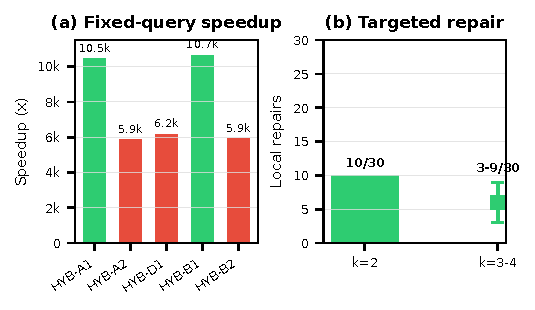
\includegraphics[width=\columnwidth]{figures/fig_hybrid_benchmark.pdf}
\caption{Hybrid benchmark results: 40 planted communities on 26K-node real DBLP. At $k$=2, \DynaSCSH repairs 10/30 targeted community-edge deletions locally with 0 recomputes.}
\Description{Hybrid benchmark plot showing fixed-query random-stream speedups and targeted local-repair success on a 26K-node planted DBLP graph.}
\label{fig:hybrid}
\end{figure}

We evaluate \DynaSCSH on the hybrid graph (26,850 nodes, 128,227 edges)---the Planted Community Benchmark combining real DBLP topology with 40 dense planted communities---under the fixed-query implementation to answer: (1) does the framework scale to 100K-edge graphs, and (2) how does incremental maintenance behave at realistic scale?

\textbf{Scaling of the speedup advantage.} Table~\ref{tab:hybrid} reports results across five experiment configurations. The hybrid runs maintain sub-millisecond dynamic latency on 128K edges. Static recomputation averages $\approx$900--944~ms, while DynaSCSH's incremental path remains below 0.16~ms on average. On insertion streams, \DynaSCSH achieves perfect community identity (Jaccard=1.000, \qratio=1.000, speedup 10,500--10,700$\times$). On deletion streams, community identity is preserved (Jaccard=1.000) with aggregate \qratio 0.933--0.934 and speedup 5,900--6,200$\times$.

\begin{table}[htbp]
\centering
\caption{Hybrid graph results under fixed-query implementation (26,850 nodes, 128,227 edges).}
\label{tab:hybrid}
\resizebox{\columnwidth}{!}{%
\begin{tabular}{c c c c c c}
\toprule
Run & $k$ & Type & Speedup & Jaccard & \qratio \\
\midrule
HYB-A1 & 2 & insertion & 10,451$\times$ & 1.000 & 1.000 \\
HYB-A2 & 2 & deletion & 5,853$\times$ & 1.000 & 0.934 \\
HYB-D1 & 3 & deletion & 6,160$\times$ & 1.000 & 0.933 \\
HYB-B1 & 2 & insertion & 10,654$\times$ & 1.000 & 1.000 \\
HYB-B2 & 2 & deletion & 5,921$\times$ & 1.000 & 0.934 \\
\bottomrule
\end{tabular}%
}
\end{table}

\textbf{Community continuity under fixed query.} The fixed-query implementation reveals a clean aggregate pattern: insertion streams preserve exact community identity, and the reported hybrid deletion runs also preserve Jaccard=1.000 while showing lower cohesiveness than the static greedy baseline (\qratio 0.933--0.934). Four fallback recomputations are recorded in each hybrid deletion summary, triggered by the strict invariant checker when local repair cannot find a valid replacement.

\textbf{Repair at scale.} To isolate repair performance, we constructed a targeted repair experiment: 30 targeted deletions from community edges at each $k$ level. Table~\ref{tab:hybrid_repair} reports the results. At $k$=2, 10 out of 30 targeted deletions were repaired locally with 0 recomputes---the larger graph provides a richer candidate pool. At higher $k$, stricter truss constraints reduce repair success and increase fallback.

\begin{table}[htbp]
\centering
\caption{Targeted hybrid repair test (30 community-edge deletions per $k$ level).}
\label{tab:hybrid_repair}
\begin{tabular}{c c c c}
\toprule
$k$ & Targeted deletions & Local repairs & Recomps \\
\midrule
2 & 30 & 10 & 0 \\
3--4 & 30 each & 3--9 & 6--9 \\
\bottomrule
\end{tabular}
\end{table}

\textbf{Q3 answered:} \DynaSCSH scales to 128K-edge graphs in the reported hybrid benchmark. Under the fixed-query implementation, insertion streams preserve community identity at 10,000$\times$+ speedup; deletion streams preserve identity with aggregate \qratio near 0.93. Localized repair succeeds at moderate $k$ on sufficiently large graphs. The speedup grows with graph scale because validation and cache maintenance are independent of the full graph size once affected projected-edge supports have been updated, while static recomputation scales with $|E|$.

\subsection{Discussion: The Cost of Dynamism}

\DynaSCSH's design follows a classic database systems principle: optimize for the common case (random updates) while maintaining acceptable behavior under targeted deletions. The three-tier performance profile is: graph-size independent validation for most updates, bounded-hop repair for community-edge hits, and fixed-query greedy recomputation when local validation fails. The hybrid graph experiments further suggest that the speedup advantage is not a constant but a function of graph scale: as graphs grow, the gap between incremental updates and full recomputation widens, making the case for dynamic maintenance increasingly compelling at deployment scale.
